% Created by tikzDevice version 0.10.1 on 2016-12-17 11:18:50
% !TEX encoding = UTF-8 Unicode
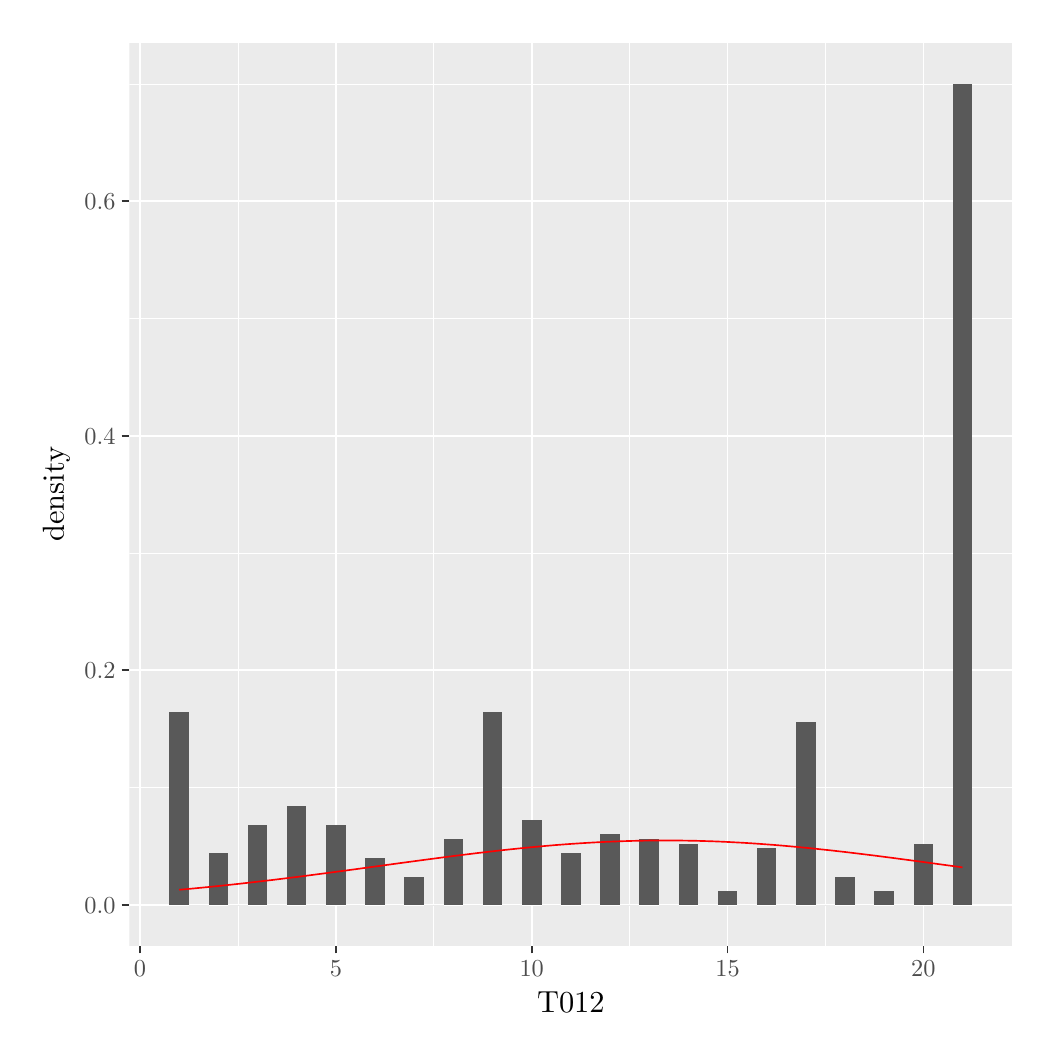
\begin{tikzpicture}[x=1pt,y=1pt]
\definecolor{fillColor}{RGB}{255,255,255}
\path[use as bounding box,fill=fillColor,fill opacity=0.00] (0,0) rectangle (361.35,361.35);
\begin{scope}
\path[clip] (  0.00,  0.00) rectangle (361.35,361.35);
\definecolor{drawColor}{RGB}{255,255,255}
\definecolor{fillColor}{RGB}{255,255,255}

\path[draw=drawColor,line width= 0.6pt,line join=round,line cap=round,fill=fillColor] (  0.00, -0.00) rectangle (361.35,361.35);
\end{scope}
\begin{scope}
\path[clip] ( 36.71, 29.59) rectangle (355.85,355.85);
\definecolor{fillColor}{gray}{0.92}

\path[fill=fillColor] ( 36.71, 29.59) rectangle (355.85,355.85);
\definecolor{drawColor}{RGB}{255,255,255}

\path[draw=drawColor,line width= 0.3pt,line join=round] ( 36.71, 86.79) --
	(355.85, 86.79);

\path[draw=drawColor,line width= 0.3pt,line join=round] ( 36.71,171.53) --
	(355.85,171.53);

\path[draw=drawColor,line width= 0.3pt,line join=round] ( 36.71,256.28) --
	(355.85,256.28);

\path[draw=drawColor,line width= 0.3pt,line join=round] ( 36.71,341.02) --
	(355.85,341.02);

\path[draw=drawColor,line width= 0.3pt,line join=round] ( 75.98, 29.59) --
	( 75.98,355.85);

\path[draw=drawColor,line width= 0.3pt,line join=round] (146.75, 29.59) --
	(146.75,355.85);

\path[draw=drawColor,line width= 0.3pt,line join=round] (217.51, 29.59) --
	(217.51,355.85);

\path[draw=drawColor,line width= 0.3pt,line join=round] (288.27, 29.59) --
	(288.27,355.85);

\path[draw=drawColor,line width= 0.6pt,line join=round] ( 36.71, 44.42) --
	(355.85, 44.42);

\path[draw=drawColor,line width= 0.6pt,line join=round] ( 36.71,129.16) --
	(355.85,129.16);

\path[draw=drawColor,line width= 0.6pt,line join=round] ( 36.71,213.90) --
	(355.85,213.90);

\path[draw=drawColor,line width= 0.6pt,line join=round] ( 36.71,298.65) --
	(355.85,298.65);

\path[draw=drawColor,line width= 0.6pt,line join=round] ( 40.60, 29.59) --
	( 40.60,355.85);

\path[draw=drawColor,line width= 0.6pt,line join=round] (111.37, 29.59) --
	(111.37,355.85);

\path[draw=drawColor,line width= 0.6pt,line join=round] (182.13, 29.59) --
	(182.13,355.85);

\path[draw=drawColor,line width= 0.6pt,line join=round] (252.89, 29.59) --
	(252.89,355.85);

\path[draw=drawColor,line width= 0.6pt,line join=round] (323.65, 29.59) --
	(323.65,355.85);
\definecolor{fillColor}{gray}{0.35}

\path[fill=fillColor] ( 51.22, 44.42) rectangle ( 58.29,113.91);

\path[fill=fillColor] ( 58.29, 44.42) rectangle ( 65.37, 44.42);

\path[fill=fillColor] ( 65.37, 44.42) rectangle ( 72.45, 63.06);

\path[fill=fillColor] ( 72.45, 44.42) rectangle ( 79.52, 44.42);

\path[fill=fillColor] ( 79.52, 44.42) rectangle ( 86.60, 73.23);

\path[fill=fillColor] ( 86.60, 44.42) rectangle ( 93.68, 44.42);

\path[fill=fillColor] ( 93.68, 44.42) rectangle (100.75, 80.01);

\path[fill=fillColor] (100.75, 44.42) rectangle (107.83, 44.42);

\path[fill=fillColor] (107.83, 44.42) rectangle (114.90, 73.23);

\path[fill=fillColor] (114.90, 44.42) rectangle (121.98, 44.42);

\path[fill=fillColor] (121.98, 44.42) rectangle (129.06, 61.37);

\path[fill=fillColor] (129.06, 44.42) rectangle (136.13, 44.42);

\path[fill=fillColor] (136.13, 44.42) rectangle (143.21, 54.59);

\path[fill=fillColor] (143.21, 44.42) rectangle (150.29, 44.42);

\path[fill=fillColor] (150.29, 44.42) rectangle (157.36, 68.15);

\path[fill=fillColor] (157.36, 44.42) rectangle (164.44, 44.42);

\path[fill=fillColor] (164.44, 44.42) rectangle (171.51,113.91);

\path[fill=fillColor] (171.51, 44.42) rectangle (178.59, 44.42);

\path[fill=fillColor] (178.59, 44.42) rectangle (185.67, 74.92);

\path[fill=fillColor] (185.67, 44.42) rectangle (192.74, 44.42);

\path[fill=fillColor] (192.74, 44.42) rectangle (199.82, 63.06);

\path[fill=fillColor] (199.82, 44.42) rectangle (206.90, 44.42);

\path[fill=fillColor] (206.90, 44.42) rectangle (213.97, 69.84);

\path[fill=fillColor] (213.97, 44.42) rectangle (221.05, 44.42);

\path[fill=fillColor] (221.05, 44.42) rectangle (228.12, 68.15);

\path[fill=fillColor] (228.12, 44.42) rectangle (235.20, 44.42);

\path[fill=fillColor] (235.20, 44.42) rectangle (242.28, 66.45);

\path[fill=fillColor] (242.28, 44.42) rectangle (249.35, 44.42);

\path[fill=fillColor] (249.35, 44.42) rectangle (256.43, 49.50);

\path[fill=fillColor] (256.43, 44.42) rectangle (263.51, 44.42);

\path[fill=fillColor] (263.51, 44.42) rectangle (270.58, 64.76);

\path[fill=fillColor] (270.58, 44.42) rectangle (277.66, 44.42);

\path[fill=fillColor] (277.66, 44.42) rectangle (284.73,110.52);

\path[fill=fillColor] (284.73, 44.42) rectangle (291.81, 44.42);

\path[fill=fillColor] (291.81, 44.42) rectangle (298.89, 54.59);

\path[fill=fillColor] (298.89, 44.42) rectangle (305.96, 44.42);

\path[fill=fillColor] (305.96, 44.42) rectangle (313.04, 49.50);

\path[fill=fillColor] (313.04, 44.42) rectangle (320.12, 44.42);

\path[fill=fillColor] (320.12, 44.42) rectangle (327.19, 66.45);

\path[fill=fillColor] (327.19, 44.42) rectangle (334.27, 44.42);

\path[fill=fillColor] (334.27, 44.42) rectangle (341.34,341.02);
\definecolor{drawColor}{RGB}{255,0,0}

\path[draw=drawColor,line width= 0.6pt,line join=round] ( 54.76, 49.83) --
	( 57.59, 50.08) --
	( 60.42, 50.35) --
	( 63.25, 50.62) --
	( 66.08, 50.90) --
	( 68.91, 51.19) --
	( 71.74, 51.49) --
	( 74.57, 51.79) --
	( 77.40, 52.10) --
	( 80.23, 52.42) --
	( 83.06, 52.75) --
	( 85.89, 53.08) --
	( 88.72, 53.41) --
	( 91.55, 53.76) --
	( 94.38, 54.11) --
	( 97.21, 54.46) --
	(100.04, 54.82) --
	(102.87, 55.19) --
	(105.71, 55.56) --
	(108.54, 55.93) --
	(111.37, 56.31) --
	(114.20, 56.69) --
	(117.03, 57.07) --
	(119.86, 57.45) --
	(122.69, 57.84) --
	(125.52, 58.23) --
	(128.35, 58.61) --
	(131.18, 59.00) --
	(134.01, 59.39) --
	(136.84, 59.77) --
	(139.67, 60.15) --
	(142.50, 60.53) --
	(145.33, 60.91) --
	(148.16, 61.28) --
	(150.99, 61.65) --
	(153.82, 62.02) --
	(156.65, 62.37) --
	(159.48, 62.72) --
	(162.31, 63.07) --
	(165.15, 63.40) --
	(167.98, 63.73) --
	(170.81, 64.05) --
	(173.64, 64.36) --
	(176.47, 64.65) --
	(179.30, 64.94) --
	(182.13, 65.22) --
	(184.96, 65.48) --
	(187.79, 65.73) --
	(190.62, 65.97) --
	(193.45, 66.19) --
	(196.28, 66.40) --
	(199.11, 66.59) --
	(201.94, 66.77) --
	(204.77, 66.93) --
	(207.60, 67.08) --
	(210.43, 67.21) --
	(213.26, 67.32) --
	(216.09, 67.42) --
	(218.92, 67.50) --
	(221.76, 67.56) --
	(224.59, 67.61) --
	(227.42, 67.64) --
	(230.25, 67.65) --
	(233.08, 67.64) --
	(235.91, 67.62) --
	(238.74, 67.57) --
	(241.57, 67.52) --
	(244.40, 67.44) --
	(247.23, 67.35) --
	(250.06, 67.24) --
	(252.89, 67.11) --
	(255.72, 66.96) --
	(258.55, 66.81) --
	(261.38, 66.63) --
	(264.21, 66.44) --
	(267.04, 66.23) --
	(269.87, 66.02) --
	(272.70, 65.78) --
	(275.53, 65.53) --
	(278.37, 65.27) --
	(281.20, 65.00) --
	(284.03, 64.72) --
	(286.86, 64.42) --
	(289.69, 64.12) --
	(292.52, 63.80) --
	(295.35, 63.48) --
	(298.18, 63.14) --
	(301.01, 62.80) --
	(303.84, 62.45) --
	(306.67, 62.10) --
	(309.50, 61.73) --
	(312.33, 61.37) --
	(315.16, 60.99) --
	(317.99, 60.62) --
	(320.82, 60.24) --
	(323.65, 59.86) --
	(326.48, 59.47) --
	(329.31, 59.08) --
	(332.14, 58.70) --
	(334.98, 58.31) --
	(337.81, 57.92);
\end{scope}
\begin{scope}
\path[clip] (  0.00,  0.00) rectangle (361.35,361.35);
\definecolor{drawColor}{gray}{0.30}

\node[text=drawColor,anchor=base east,inner sep=0pt, outer sep=0pt, scale=  0.88] at ( 31.76, 41.39) {0.0};

\node[text=drawColor,anchor=base east,inner sep=0pt, outer sep=0pt, scale=  0.88] at ( 31.76,126.13) {0.2};

\node[text=drawColor,anchor=base east,inner sep=0pt, outer sep=0pt, scale=  0.88] at ( 31.76,210.87) {0.4};

\node[text=drawColor,anchor=base east,inner sep=0pt, outer sep=0pt, scale=  0.88] at ( 31.76,295.62) {0.6};
\end{scope}
\begin{scope}
\path[clip] (  0.00,  0.00) rectangle (361.35,361.35);
\definecolor{drawColor}{gray}{0.20}

\path[draw=drawColor,line width= 0.6pt,line join=round] ( 33.96, 44.42) --
	( 36.71, 44.42);

\path[draw=drawColor,line width= 0.6pt,line join=round] ( 33.96,129.16) --
	( 36.71,129.16);

\path[draw=drawColor,line width= 0.6pt,line join=round] ( 33.96,213.90) --
	( 36.71,213.90);

\path[draw=drawColor,line width= 0.6pt,line join=round] ( 33.96,298.65) --
	( 36.71,298.65);
\end{scope}
\begin{scope}
\path[clip] (  0.00,  0.00) rectangle (361.35,361.35);
\definecolor{drawColor}{gray}{0.20}

\path[draw=drawColor,line width= 0.6pt,line join=round] ( 40.60, 26.84) --
	( 40.60, 29.59);

\path[draw=drawColor,line width= 0.6pt,line join=round] (111.37, 26.84) --
	(111.37, 29.59);

\path[draw=drawColor,line width= 0.6pt,line join=round] (182.13, 26.84) --
	(182.13, 29.59);

\path[draw=drawColor,line width= 0.6pt,line join=round] (252.89, 26.84) --
	(252.89, 29.59);

\path[draw=drawColor,line width= 0.6pt,line join=round] (323.65, 26.84) --
	(323.65, 29.59);
\end{scope}
\begin{scope}
\path[clip] (  0.00,  0.00) rectangle (361.35,361.35);
\definecolor{drawColor}{gray}{0.30}

\node[text=drawColor,anchor=base,inner sep=0pt, outer sep=0pt, scale=  0.88] at ( 40.60, 18.58) {0};

\node[text=drawColor,anchor=base,inner sep=0pt, outer sep=0pt, scale=  0.88] at (111.37, 18.58) {5};

\node[text=drawColor,anchor=base,inner sep=0pt, outer sep=0pt, scale=  0.88] at (182.13, 18.58) {10};

\node[text=drawColor,anchor=base,inner sep=0pt, outer sep=0pt, scale=  0.88] at (252.89, 18.58) {15};

\node[text=drawColor,anchor=base,inner sep=0pt, outer sep=0pt, scale=  0.88] at (323.65, 18.58) {20};
\end{scope}
\begin{scope}
\path[clip] (  0.00,  0.00) rectangle (361.35,361.35);
\definecolor{drawColor}{RGB}{0,0,0}

\node[text=drawColor,anchor=base,inner sep=0pt, outer sep=0pt, scale=  1.10] at (196.28,  5.50) {T012};
\end{scope}
\begin{scope}
\path[clip] (  0.00,  0.00) rectangle (361.35,361.35);
\definecolor{drawColor}{RGB}{0,0,0}

\node[text=drawColor,rotate= 90.00,anchor=base,inner sep=0pt, outer sep=0pt, scale=  1.10] at ( 13.08,192.72) {density};
\end{scope}
\end{tikzpicture}
